
\documentclass{article}

% For figures
\usepackage{graphicx} 

% For citations
\usepackage{natbib}

% For algorithms
\usepackage{algorithm}
\usepackage{algorithmic}

% As of 2010, we use the hyperref package to produce hyperlinks in the
% resulting PDF.  If this breaks your system, please commend out the
% following usepackage line and replace \usepackage{icml2010} with
% \usepackage[nohyperref]{icml2010} above.
\usepackage{hyperref}

% Packages hyperref and algorithmic misbehave sometimes.  We can fix
% this with the following command.
\newcommand{\theHalgorithm}{\arabic{algorithm}}
\usepackage[accepted]{icml2010}


% The \icmltitle you define below is probably too long as a header.
% Therefore, a short form for the running title is supplied here:
\icmltitlerunning{Title}

\begin{document} 

\twocolumn[
\icmltitle{Using Bayesian networks to predict changes}


\icmlauthor{Sarah Nadi}{snadi@uwaterloo.ca}
\icmladdress{University of Waterloo,
            Waterloo, ON, Canada}

\vskip 0.3in
]

\begin{abstract} 
STILLLL
\end{abstract} 

\section{Introduction}
\label{intro}

Changes

\section{Background}

\subsection{CMDBs and Change Sets}
A Configuration Management Database (CMDB) is useful in Enterprise IT Management (EITM) since it provides information about the various critical components in a
system including hardware, software, and services provided by the company. It records the configuration of these items, their change history, their incident
history, as well as the relationships between them. Each item stored in the CMDB is referred to as a Configuration Item (CI). Figure~\ref{fig:cmdbExample} shows
an example CMDB to illustrate the concepts of CIs and relationships. In this example, there are two software applications being hosted by two different web
servers. Both applications communicate with the same databases through a load balancer. Such a visualization allows an IT analyst to better understand the
system at hand.

A CMDB provides a basis for decision making processes such as Incident Management, Change Management, etc.  In this paper, we focus on the process of Change
Management, and in particular, on the problem of change set detection .A \textit{change} is the addition, modification, or removal of anything that could affect
on IT services. A poorly planned change may lead to a fault in the system. Accordingly, when one wants to change one CI is the system, other CIs that might
need to be changed as well must be correctly identified. The set of CIs that will need to be modified for the change to be complete is called a change set.

\begin{figure}[!t]
\centering
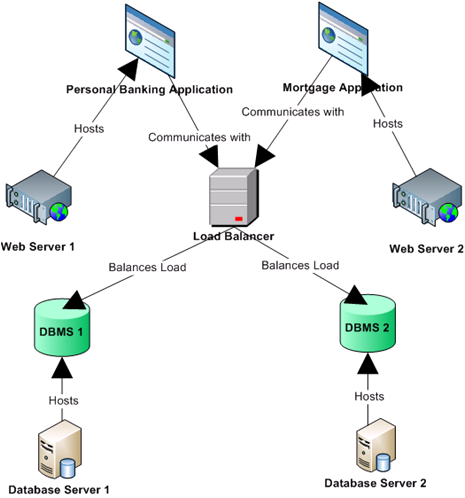
\includegraphics[width=7cm]{cmdbExample.PNG}
\caption{An IT System Stored in a CMDB}
\label{fig:cmdbExample}
\end{figure}

\subsection{Bayesian Networks}

\subsubsection{Tools}

\subsubsection*{Weka}

\subsubsection*{Banjo}
Banjo is a tool written in Java which infers the structure of a Bayesian network given training data. It has two different search algorithms: Greedy and
Simulated Annealing. For either of these search algorithms, it has two methods of proposing a new edge. The first is the ``proposeRandomLocalMove''
which basically proposes a random addition or removal of an edge. The other is ``proposeAllLocalMoves'' which proposes all possible moves, and only keeps the
best one (?). Banjo uses the BDe metric to compute a network's score.

\subsubsection*{JavaBayes}

\subsection{Evaluation Techniques}

We need a way to evaluate the predicted CIs. The recall and precision measures from the information retrieval field are appropriate for this type of evaluation.
Recall measures the proportion of correct CIs retrieved by the system, while precision measures the proportion of suggested CIs that are correct~\cite{van79}.

Similar to Hassan et. al~\cite{hassan2004predicting}, we define the \textit{Predicted Set} (P) as the set of all CIs DRACA suggests through the full the
iteration process (see Figure~\ref{fig:process}). We define the \textit{Occurred Set} (O) as the CIs remaining in the change set after excluding the Initial CI
provided by the analyst (i.e Change Set - Initial CI). The intersection of the predicted set and the occurred set, called $PO$, is the common CIs in both sets.
For each constructed change set, we then calculate the recall and precision values for the predictions according to the following
definitions~\cite{hassan2004predicting}:

\begin{equation}
\label{eqn:recall}
Recall = \frac{|PO|}{|O|}
\end{equation}

\begin{equation}
\label{eqn:precision}
Precision = \frac{|PO|}{|P|}
\end{equation}

If no CIs are predicted (i.e., $P$ and thus $PO$ are empty), precision is defined as 1 since there cannot exist any incorrect predictions in an empty set. On
the other hand, if the size of the change set is 1, and thus the size of the occurred set is 0, recall is defined as 1 since there are no CIs to
predict~\cite{hassan2004predicting}.  

In order to have a single measure that indicates the effectiveness of our predictions, we use the F-measure which is based on van Rijsbergen's effectiveness
measure which combines recall and precision~\cite{van79}. The F-measure is calculated according to Equation~\ref{eqn:f-measure} which gives equal weighting to
recall and precision. The ideal F-measure is 1 where both recall and precision are 1.

\begin{equation}
F = 2 * \frac{precision * recall}{precision +recall}
\label{eqn:f-measure}
\end{equation}

\section{Related Work}
\label{rel-work}

Mirarab et al.~\cite{mirarab2007} investigate the same problem as our work. However, their work is on the level of source code changes. They build three
different Bayesian Networks, one that is based on package and class dependency information (static relationships), one which is dependent on historical
co-changes, and one which uses both. For the first graph, the initial structure is essentially ``given'' according to the static dependencies, and then the CPTs
are learnt using the importance sampling algorithm proposed by Changhe and Marek~\cite{yuan2003importance}. The way static dependencies are defined in their
case is specific to Java. The third one is essentially the first graph, but updated using the historic change information according to the Expectation
Maximization (EM) algorithm~\cite{dempster1977maximum}. The second was solely based on historic information where the network is build using a greedy structure
 learning algorithm~\cite{friedman1996learning}. They did some preprocessing to their data such as filtering out large changes (with more than 30 elements
changed at once) since this was probably an insignificant change.

Zhou et al.~\cite{zhou2008} try to answer a slightly different problem. They do not only look at the probability of other elements changing given a specific
element, they also add features such as authors, change significance levels etc. and try to predict if two elements are co-changes or not accordingly. Thus,
their problem is more of a classification problem where given two elements, and some observed features they try to determine the class as co-changes or not.
They use the K2 algorithm proposed by Cooper et. al~\cite{cooper1992bayesian} to estimate the structure of the Bayesian network, and use the SimpleEstimator
algorithm built in WEKA~\cite{witten2005data}.

\section{Models Used}
\label{sec:modelsused}

We experimented with several models to predict change sets. First, we just used Weka's BayesNet classifier to build the structure and estimate the CPTs of
the network. In the second model, we used Banjo to learn the structure of the network, and then we used Weka to learn the CPTs. In the third model, we imposed
the structure of the network from the relationships already existing between CIs in the CMDB. Finally, in the fourth model, we tried to assume that CIs not in
a change order are unobserved data, and therefore have missing values.

In order to be able to test things properly, we chose a small dataset to be able to build our model. We used observations from three months data from January 1,
2008 to March 31, 2008 to build the model. However, in such a short period, there were already 2,841 distinct CIs appearing and 2,229 observations (i.e. change
orders). Therefore, in each model, some data preprocessing was done before building the model since having a network with over 2000 variables was very hard to
deal with.

\subsection{Model 1}
\label{sec:model1}


\subsection{Model 2}
\label{sec:model2}

\subsubsection*{Data Preprocessing}

For this model, we first got a list of all the CIs that appeared more than 12 times (i.e were associated with 12 different change orders in our training
observations). This yielded 120 distinct CIs. Then, in order to slightly increase our variable space to include other related CIs, we found all the parent CIs
related to these 120 CIs from the CMDB perspective. However, we ignored three common, and not extremely meaningful relations, which are  ``supports'', ``is
location for'', and ``backs up''. Adding the related parent CIs, we now had a set of 241 CIs. We then went back, and iterated through the observations, and
kept only observations for CIs that either had more than 12 different change orders or were related to these CIs (i.e that occurred in the set of 241 CIs).
This, finally, gave us a set of 170 distinct CIs which we used for our model. Additionally, filtering out CIs meant filtering out some of the observations that
did not have any CIs satisfying our criteria. This led to us having 1305 observations instead of 2841 which was a more manegeable set.

\subsubsection*{Building the Model}

Given that we had our training set, the next step was to build the network which has two parts: building the structure, and estimating the CPTs. Unfortunately,
Weka mainly focused on classification and clustering which is not exactly the same problem we are tackling here. However, Weka did provide a functionality to
learn the CPT of a network given a certain structure. We, therefore, used Banjo to build the structure of the network (Banjo does not estimate CPTs), and then
used Weka to estimate the CPTs on the produced network. In both cases, the same observations file was used to ensure that its the same data. However, each tool
accepted the data in different formats, so some translation was necessary there. After Weka has added the CPT information to the graph, we used this as the
final Bayesian network on which to do our analysis.

\subsubsection*{Inference}

At this point, we have the Bayesian network ready, and we would like to perform Inference. More formally, given that a CI will change (our evidence), we want
to infer the probability that the other CIs in the network might change as well. Unfortunately, neither of the two tools previously used provide an Bayesian
inference engine. We, therefore, use JavaBayes in this step since it accepts the same ARFF format used by Weka. We using a one month testing set where we try
to predict all the change orders in April 2008 (883 reports). There was a total of XX change orders in that month. For each change order, we would take the
first CI as the initial CI to change, then we would set that as evidence, and update the beliefs of all the nodes (CIs) in the network using JavaBayes. We would
then loop on all the updated CIs, and add those that match our threshold criteria to the predicted change set. To simulate a real life scenario, we then checked
which of these predicted CIs actually lies in the target change set we are trying to predict. This is similar to an analyst accepting CIs into their change set.
These common CIs would then also be marked as observations so that we can predict now that I'm going to change B and C too, what else do I need to change.
Again, we would calculate the posterior probability, and continue doing so until there are no more common CIs. We would then calculate the recall, precision,
and F-measure accordingly.

\subsubsection*{Results}


\subsection{Model 3}

\subsubsection*{Data Preprocessing}

For this model, we only used the list of CIs appearing more than 12 times (120 distinct CIs). 

\subsubsection*{Building the Model}

Using CIs in this list only, we constructed the structure of the Bayesian network by adding in CMDB relationships between the CIs. We stuck to this set only to
ensure that all the CIs in the network, are also present in the observations. Fourty-eight edges were added to the structure of the network. Using these 120
CIs, we had XXX observations. Again, we loaded the produced structure in Weka, and learned the CPTs using the observations from the three months. We then took
the produced Bayesian network, and used JavaBayes to perform the inference.

\subsubsection*{Inference}



\section{Building the model}
\label{sec:model}

\section{Experimental Work}
\label{sec:exp}

\section{Conclusion}
\label{concl}


\bibliography{references}
\bibliographystyle{icml2010}

\end{document} 


